%%%%%%%%%%%%%%%%%%%%%%%%%%%%%%%%%%%%%%%%%%%%%%%%%%%%%%%%%%%%%%%%%%%%%%%%%%%%%%%%%
%
% Philipp's part
%
%%%%%%%%%%%%%%%%%%%%%%%%%%%%%%%%%%%%%%%%%%%%%%%%%%%%%%%%%%%%%%%%%%%%%%%%%%%%%%%%%
\section{}
\subsection{State of the art method, Time of flight:}
\begin{frame}{State of the art method, Time of flight:}

Using (varying) active illumination and reconstructing a scene from multiple images\\
Shortcomings:
\begin{itemize}
\item Low mapping rate (~30Hz)
\item Motion artifacts
\item Multipath-interference
\end{itemize}

\end{frame}

\begin{frame}{Examples}
\begin{figure}
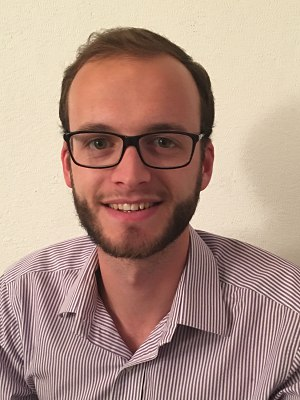
\includegraphics[scale=0.9]{pictures/polop}
\caption{Examples}
\end{figure}
\end{frame}

%%%%%%%%%%%%%%%%%%%%%%%%%%%%%%%%%%%%%%%
\subsection{State of the art method, Structured Light:}
\begin{frame}{State of the art method, Structured Light:}

Spatial patterns projected on the scene\\
Shortcomings:
\begin{itemize}
\item Robustness issues
\item Motion artifacts
\item Limited depth-range
\item Overlapping sensors cause interference
\end{itemize}

\end{frame}

\begin{frame}{Examples}
\begin{figure}
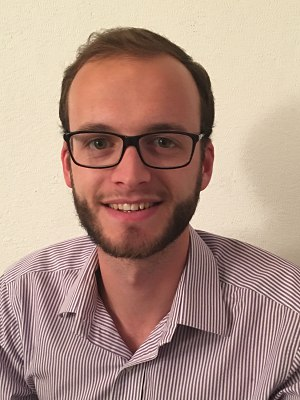
\includegraphics[scale=0.9]{pictures/polop}
\caption{Examples}
\end{figure}
\end{frame}

%%%%%%%%%%%%%%%%%%%%%%%%%%%%%%%%%%%%%%%%

\subsection{Solution to a lot of these issues: Active Stereo:}
\begin{frame}{Solution to a lot of these issues: Active Stereo:}

Using 2 calibrated cameras and 1 pattern-projecting light source

\begin{itemize}
\item Mitigates multipath reflections
\item Improves robustness
\item Avoids interference between multiple systems\\
\item BUT correspondence search has high computational cost
\end{itemize}

\end{frame}

\begin{frame}{Examples}
\begin{figure}
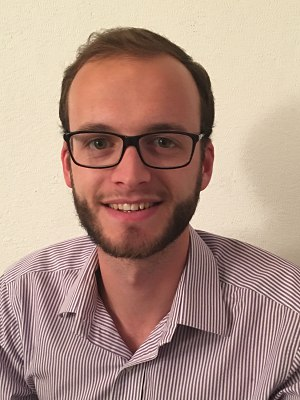
\includegraphics[scale=0.9]{pictures/polop}
\caption{Examples}
\end{figure}
\end{frame}
